\documentclass[a4paper,10pt]{article}
\usepackage[hidelinks]{hyperref}
\def\UrlBreaks{\do\/\do-} % breaks long url in references
\usepackage{graphicx}
\usepackage[english]{babel}
\usepackage{listings}
\usepackage[labelfont=it,textfont={it},singlelinecheck=on,justification=centering]{caption}
\usepackage{amsmath}
\usepackage{float}

\lstset{basicstyle=\ttfamily\footnotesize,breaklines=true}
\lstset{numbers=left, numberstyle=\tiny, stepnumber=1, numbersep=5pt}
\lstset{language=TeX}
\setlength{\parskip}{1em}
\renewcommand{\baselinestretch}{1.2}

\title{\textbf{Storj\\A Peer-to-Peer Cloud Storage Network}}
\author{\\
Shawn Wilkinson (shawn@storj.io),\\
Tome Boshevski (tome@storj.io),\\
Josh Brandoff (josh.brandoff@gmail.com),\\
James Prestwich (james@storj.io),\\
Gordon Hall (gordonhall@openmailbox.org),\\
Patrick Gerbes (patrickgerbes@gmail.com)\\
\\
With contributions from: Vitalik Buterin (v@buterin.com)
}
\date {December 15, 2016 \\ v2.0}

\begin{document}
\maketitle
\begin{abstract}
A peer-to-peer cloud storage network implementing client-side encryption would allow users to transfer and share data without reliance on a third party storage provider. The removal of central controls would mitigate most traditional data failures and outages, as well as significantly increase security, privacy, and data control. Peer-to-peer networks are generally unfeasible for production storage systems, as data availability is a function of popularity, rather than utility. We propose a solution in the form of a challenge-response verification system coupled with direct payments. In this way we can periodically check data integrity, and offer rewards to peers maintaining data. We further propose a model for addressing access and performance concerns with a set of independent or federated nodes.
\end{abstract}


\section{Introduction}
Cloud storage has come to rely almost exclusively on storage providers acting as trusted third parties to transfer and store data. While this system works in most cases, it still suffers from the inherent weaknesses of a trust-based model. Because client-side encryption is nonstandard, the traditional cloud is vulnerable to a variety of security threats, including man-in-the-middle attacks, malware, and application flaws that expose private consumer and corporate data. Furthermore, current cloud storage providers charge large markups over the core costs of data storage hardware in order to maintain expensive infrastructure. Moreover, because many storage devices rely on the same infrastructure, the impact of any failure is magnified.

A decentralized cloud storage network offers many advantages compared to datacenter-based cloud storage. Data security can be maintained using client-side encryption, while data integrity will be maintained via a proof of retrievability. The impact of infrastructure failures and security breaches will be greatly reduced. An open market for data storage may drive down costs for various storage services by enabling more parties to compete using existing devices. Data on the network will be resistant to censorship, tampering, unauthorized access, and data failures. This paper describes a concrete implementation of such a network, and a set of tools for interacting with that network.


\section{Design}
Storj is a protocol that creates a distributed network for the formation and execution of storage contracts between peers. The Storj protocol enables peers on the network to negotiate contracts, transfer data, verify the integrity and availability of remote data, retrieve data, and pay other nodes. Each peer is an autonomous agent, capable of performing these actions without significant human intervention. Many of the basic tools for these interactions are described here. Full protocol documentation can be found elsewhere \cite{1}.

\subsection{Files as Encrypted Shards}
A shard is a portion of a file consisting of $ S $ bytes to be stored on this network. Sharding has a number of advantages to security, privacy, performance, and availability.

Shards should be independently encrypted client-side before entering the network. The reference implementation uses AES256-CTR, but convergent encryption or any other desirable system could be implemented. This protects the content of the data from the storage provider, or ‘farmer,’ housing the data. The data owner retains complete control over the encryption key, and thus over access to the data.

The data owner may separately secure knowledge of how a file is sharded and where in the network the shards are located. As the set of shards in the network grows, it becomes exponentially more difficult to locate any given shard set without prior knowledge of their locations (see Section 6.3). This implies that security of the file is proportional to the square of the size of the network.

Shard size is a negotiable contract parameter. To preserve privacy, it is recommended that shard sizes be standardized as a byte multiple, such as 8 or 32 MB. Smaller files may be filled with zeroes or random data. Standardized sizes dissuade side-channel attempts to determine the content of a given shard, and can mask the flow of shards through the network.

Sharding large files like video content and distributing the shards across nodes reduces the impact of content delivery on any given node. Bandwidth demands are distributed more evenly across the network. In addition, the end-user can take advantage of parallel transfer, similar to BitTorrent or other peer-to-peer networks.

Because peers generally rely on separate hardware and infrastructure, data failure is not correlated. This implies that creating redundant mirrors of shards, or applying a parity scheme across the set of shards is an extremely effective method of securing availability. Availability is proportional to the number of nodes storing the data.

% TODO: Graphic

\begin{enumerate}
\item Files are split into shards, or multiple files are combined to form a shard.
\item Each shard is encrypted.
\item Audit pre-processing is performed for each shard (see Section 2.3).
\item Shards are transmitted to the network.
\end{enumerate}

\subsection{Kademlia and Modifications}
Storj is built on a Kademlia \cite{2}, a distributed hash table. It is important to note that shards are not stored in the hash table. Rather, Kademlia creates a distributed network with efficient message routing and other desirable qualities. Storj adds several message types, and enhancements to core Kademlia functionality. In the future, the hash table may be used as a store for data location information, or other purposes.

\subsubsection{Signature Verification}
Similar to S/Kademlia \cite{3}, the Storj network requires peers to sign messages. To join the network a node must create an ECDSA keypair, $ (k_{priv}, k_{pub}) $. The Kademlia Node ID corresponds to $ ripemd160(sha256(k_{pub})) $. As such, each Node ID in the Storj network is also a valid Bitcoin address, which the node can spend from. Nodes sign all messages, and validate message signatures before processing messages. This modification enforces long-term identity on the network, and provides a proof of work deterrent to Sybil and Eclipse attacks on Kademlia routing. In the future there are a variety of other uses for this address.

\subsection{Proofs of Retrievability}
Proofs of retrievability guarantee the existence of a certain piece of data on a remote host. The ideal proof minimizes message size, can be calculated quickly, requires minimal pre-processing, and provides a high degree of confidence that the file is available and intact. To provide knowledge of data integrity and availability to the data owner, Storj provides a standard format for issuing and verifying proofs of retrievability via a challenge-response interaction called an “audit” or “heartbeat.”

Our reference implementation uses Merkle trees \cite{5} and Merkle proofs. After the sharding process the data owner generates a set of $ n $ random challenge salts $ s_{0}, s_{1}, ... s_{n-1} $ and stores the set of salts $ s $. The challenge salts are each prepended to the data $ d $, and the resulting string is hashed to form a “pre-leaf” $ p $ as such: $ p_{i} = H(s_{i} + d) $. Pre-leaves are hashed again, and the resulting digests become the set of leaves $ l $ of a standard Merkle tree such that $ l_{i} = H(H(s_{i} + d)) $. The leaf set is filled with hashes of a blank string until its length is a power of two, to simplify the proof process.

% TODO: Graphic

The data owner stores the set of challenges, the Merkle root and the depth of the Merkle tree, then transmits the Merkle tree’s leaves to the farmer. The farmer stores them along with the shard. Periodically, the data owner selects a challenge from the stored set, and transmits it to the farmer. The farmer uses the challenge and the data to generate the pre-leaf. The pre-leaf, along with the set of leaves, is used to generate a Merkle proof, which is sent back to the data owner.

The Merkle proof always consists of exactly $ log_{2}(l) $ hashes, and thus is a very compact transmission, even for large trees. The data owner uses the stored Merkle root and tree depth to verify the proof by verifying that its length is equal to the tree depth and the hashes provided recreate the stored root. This scheme does not allow false negatives or false positives, as the hash function requires each bit to remain intact to produce the same output.

\subsubsection{Partial Audits}
The Merkle tree audit scheme requires significant computational overhead for the data owner, as the entire shard must be hashed many times to generate pre-leaves. An extension of this scheme utilizes subsets of the data to perform partial audits, reducing computational overhead. This also has the advantage of significantly reducing I/O burden on farmer resources.

This extension relies on two additional selectable parameters: a byte index $ x $ within the shard and a number of bytes, $ b $. The data owner stores a set of 3-tuples $ (s, x, b) $. To generate pre-leaf $ i $, the data owner prepends $ s_{i} $ to the $ b_{i} $ bytes found at $ x_{i} $. During the audit process, the verifier transmits $ (s, x, b)_{i} $, which the farmer uses to generate a pre-leaf. The Merkle proof is generated and verified as normal.

%TODO: Graphic

Partial audits provide only probabilistic assurance that the farmer retains the entire file. They allow for false positive results, where the verifier believes the farmer retains the intact shard, when it has actually been modified or partially deleted. The probability of a false positive on an individual partial audit is easily calculable (see Section 6.4)

Thus the data owner can have a known confidence level that a shard is still intact and available. In practice, this is more complex, as farmers may implement intelligent strategies to attempt to defeat partial audits. Fortunately, this is a bounded problem in the case of iterative audits. The probability of several consecutive false positives becomes very low, even for small deletions of the file.

In addition, partial audits can be easily mixed with full audits without restructuring the Merkle tree or modifying the proof verification process. Many audit strategies that mix full and partial verification can be envisioned, each of which provides different levels of confidence over time.

A further extension of this scheme could use a deterministic seed instead of a set of byte indexes. This seed would be used to generate indexes of many non-consecutive bytes in the file. Requiring many non-consecutive random bytes would provide additional resistance against malicious farmers attempting to implement audit evasion strategies without significant extra overhead from processing or I/O.

\subsubsection{Other Proof-of-Retrievability Schemes}
Other audit schemes were examined, but deemed generally unfeasible. For example, Shacham and Waters proposed a compact proof \cite{6} with several advantages over Merkle-tree schemes. For instance, this construction allows for an endless stream of challenges to be generated by the data owner with minimal stored information. It also allows for public verifiability of challenge responses.

However, initial implementations indicate that the client-side pre-processing required for the Shacham-Waters scheme requires at least one order of magnitude more computation time than hash-based methods, rendering it too slow for most applications.

Proof of retrievability is an area of ongoing research, and other practical schemes may be discovered in the future. As proof of retrievability schemes are discovered and implemented, the choice of scheme may become a negotiable contract parameter. This would allow each data owner and node to implement a wide variety of schemes, and select the most advantageous scheme for a given purpose.

\subsubsection{Issuing Audits}
To issue audits, Storj extends the Kademlia message set with a new type: AUDIT. These messages are sent from data owners to farmers and contain the hash of the data and a challenge number. The farmer must respond with a merkle proof as described above. Upon receipt and validation of the Merkle proof, the data owner must issue payment to the farmer according to agreed-upon terms.

%TODO: Graphic

\subsection{Contracts and Negotiation}
Data storage is negotiated via a standard contract format \cite{7}. The contract is a versioned data structure that describes the relationship between data owner and farmer. Contracts should contain all information necessary for each node to form a relationship, transfer the data, create and respond to audits over time, and arbitrate payments. This includes shard hash, shard size, audit strategy, and payment information. Storj implements a publish/subscribe system to connect parties interested in forming a contract (see Section 2.6).

Each party should store a signed copy of the contract. Contracts exist solely for the benefit of the data owner and farmer, as no other node can verify the terms or state of the relationship. In the future, contract information may be stored in the DHT, or in an external ledger like a Blockchain, which may allow some outside verification of relationship terms.

The contracting system extends Kademlia with four new message types: OFFER, CONSIGN, MIRROR, and RETRIEVE.

To negotiate a contract, a node creates an OFFER message and sends it to a prospective partner. Prospective partners are found via the publish/subscribe system described in Section 2.6. The OFFER message contains a fully-constructed contract that describes the desired relationship. The two nodes repeatedly swap signed OFFER messages. For each new message in the OFFER loop, the node either chooses to terminate negotiations, respond with a new signed counter-offer, or accept the contract by countersigning it. Once an OFFER is signed by both parties, they each store it locally, keyed by the hash of the data.

Once an agreement is reached, the data owner sends a CONSIGN message to the farmer. The message contains the leaves of the audit-tree. The farmer must respond with a PUSH token that authorizes the data owner to upload the data via HTTP transfer (see Section 2.10). This token is a random number, and can be delegated to a third party.

RETRIEVE messages signify the intent to retrieve a shard from a farmer. These messages are nearly identical to CONSIGN messages, but do not contain the audit-tree leaves. The farmer responds to a valid RETRIEVE message with a PULL token that authorizes download of the data via a separate HTTP transfer.

MIRROR messages instruct a farmer to retrieve data from another farmer. This allows data owners to create redundant copies of a shard without expending significant additional bandwidth or time. After a successful OFFER/CONSIGN process, the data owner may initiate a separate OFFER loop for the same data with another farmer. Instead of issuing a CONSIGN message to the mirroring farmer, the data owner instead issues a RETRIEVE message to the original farmer, and then includes the retrieval token in a MIRROR message to the mirroring farmer. This authorizes the mirroring farmer to retrieve the data from the original farmer. The success of the MIRROR process should be verified immediately via an AUDIT message.

\subsection{Payment}
Storj is payment agnostic. Neither the protocol nor the contract requires a specific payment system. The current implementation assumes Storjcoin, but many different payment types could be implemented, including Storjcoin, BTC, Ether, ACH transfer, or physical transfer of live goats.

The reference implementation will use Storjcoin micropayment channels, which are currently under development. Micropayment channels allow for pairing of payment directly to audit, thus minimizing the amount of trust necessary between farmers and data owners. However, because data storage is inexpensive, audit payments are incredibly small, often below \$0.000001 per audit.

Storjcoin allows much more granular payments than other candidate currencies, thereby minimizing trust between parties. In addition, the mechanics of micropayment channels require the total value of the channel to be escrowed for the life of the channel. This decreases currency velocity, and implies that value fluctuations severely impact the economic incentives of micropayment channels. The use of a separate token creates a certain amount of insulation from outside volatility, and Storjcoin's large supply minimizes the impact of token escrow on the market.

New payment strategies must include a currency, a price for the storage, a price for retrieval, and a payment destination. It is strongly advised that new payment strategies consider how data owners prove payment, and farmers verify receipt without human interaction. Implementation details of other payment strategies are left as an exercise for interested parties.

\subsection{Quasar}
Storj implements a peer-to-peer publish/subscribe system called Quasar \cite{8}\cite{9}. Quasar offers topic-based pub/sub utilizing Bloom filters \cite{10}. Current topic options include size and bandwidth commitment, and the topic list is easily extensible \cite{11}. This facilitates the contract offer and negotiation process (see Section 2.4)

To operate Quasar, Storj extends Kademlia with three new message types: SUBSCRIBE, UPDATE, and PUBLISH. These messages facilitate the creation and propagation of filters. Each node maintains information about topics to which it subscribes, as well as topics to which its neighbors subscribe in the form of an attenuated Bloom filter with depth $ K = 3 $. The filter at level 1 represents the subscriptions of nodes 1 hop away.

SUBSCRIBE requests filter lists from neighbors. To build an initial filter list, nodes issue SUBSCRIBE messages to their three nearest neighbors. Nodes respond to a SUBSCRIBE with their current filter list. The requesting node adds the received filter lists to its own attenuate Bloom filter.

UPDATE pushes local filter changes to the three nearest neighbors. When a node subscribes to a new topic it must issue a SUBSCRIBE request to learn about its neighbors’ states, then an UPDATE request to notify neighbors of its new subscription. By exchanging filter lists via SUBSCRIBE/UPDATE loops nodes gain progressively better knowledge of what information is desirable to their neighbors, and to nodes reachable by their neighbors.

PUBLISH broadcasts a message to the network. In Storj, these are typically public announcements of partially-constructed contracts (see Section 2.4). PUBLISH messages are sent to a node’s three nearest neighbors, and include a topic parameter whose digest is compared to each filter in the filter list. If the topic digest is found in the filter at $ K = 0 $, the node processes the message. If the topic is found in any other filters in the filter list, the node forwards the message to its neighbors. If no matching filter is found, the message is forwarded to a randomly selected peer in that node’s routing table.

To prevent re-circulation of messages, nodes add their node ID to PUBLISH messages when they are forwarded, indicating that that node has already received the message. When forwarding messages, nodes ignore other nodes whose IDs are present in that list. This prevents redundant recirculation of messages with minimal communication overhead.

PUBLISH messages also include a time-to-live (TTL) parameter, measured in hops. Nodes will not relay messages whose hops have exceeded the TTL. To prevent spam attacks, nodes will also refuse to relay messages whose TTL exceeds the network default.

Because of this routing process based on subscription filters, PUBLISH propagate through the network randomly until they find a node whose filter list contains a subscription or a false positive. Once a subscription is indicated by a filter, the message moves towards the subscriber quickly. If a false positive is encountered the message resumes random routing.

\subsection{Redundancy Schemes}
Cloud object stores typically own or lease servers to store their customers’ files. They use RAID schemes or a multi-datacenter approach to protect the file from physical or network failure. Because Storj objects exist in a distributed network of untrusted peers, farmers should not be relied upon to employ the same safety measures against data loss as a traditional cloud storage company. Indeed, farmers may simply turn off their node at any time. As such, it is strongly recommended that the data owner implement redundancy schemes to ensure the safety of their file. Because the protocol deals only with contracts for individual shards, many redundancy schemes may be used. Three are described below.

\subsubsection{Simple Mirroring}
The simplest solution is to mirror shards across several nodes. Mirroring protects against hardware failures by ensuring that multiple copies of each shard exist. Availability of the shard with this scheme is $ P = 1 - \prod_{0}^{n} a_{n} $ where $ a_{n} $ is the uptime of the node storing shard $ n $. Because all shards are required to assemble the file, availability of the file is equal to the availability of the least available shard. In the case of a dropped contract, a redundant copy of that shard can be retrieved and a new location found for it on the network. This is the current behavior of the reference implementation.

\subsubsection{K-of-M Erasure Coding}
Storj will soon implement client-side Reed-Solomon erasure coding. Erasure coding algorithms break a file into $ k $ shards, and programmatically create $ m $ parity shards, giving a total of $ k + m = n $ shards. Any $ k $ of these $ n $ shards can be used to rebuild the file or any missing shards. Availability of the file is then $ P = 1 - \prod_{0}^{m} a_{m} $  across the set of the $m + 1$ least available nodes. In the case of loss of individual shards, the file can be retrieved, the missing shard rebuilt, and then a new contract negotiated for the missing shard.

To prevent loss of the file, data owners should set shard loss tolerance levels. Consider a 20-of-40 erasure coding scheme. A data owner might tolerate the loss of 5 shards out of 40, knowing that the chance of 16 more becoming inaccessible in the near future is low. However, at some point the probabilistic availability will fall below safety thresholds. At that point the data owner must initiate a retrieve and rebuild process.

Because node uptimes are known via the audit process, tolerance levels may be optimized based on the characteristics of the nodes involved. Many strategies may be implemented to handle this process.

Erasure coding is desirable because it drastically decreases the probability of losing access to a file. It also decreases the on-disk overhead required to achieve a given level of availability for a file. Rather than being limited by the least available shard, erasure coding schemes are limited by the least-available $ n + 1 $ nodes (see Section 6.1).

\subsection{KFS}
To facilitate on-disk storage for farmers, Storj implements a local file store called KFS \cite{12}. The farming client initially used the filesystem directly to store shards. Later the farming client used a single LevelDB instance. Both of these approaches failed to scale. For example, LevelDB compaction processing time scales linearly with store size, and locks both reads and writes while in progress. This significantly impacted performance and availability for nodes storing more than 100GB. KFS is an abstraction layer over a set of LevelDB instances that seeks to address scaling problems.

\subsubsection{Rationale}
LevelDB is a key-value store. It has many desirable qualities, including long-term support, portability, and high performing reads powered by lexicographically sorted keys. While LevelDB compaction is typically a desirable feature, it severely limits scaling. This impact is larger on lower end systems and can also vary based on the type of disk in use. Compaction also blocks reads and writes during this period, rendering Storj nodes effectively offline until the process completes.

However, because LevelDB instances are cheap to create, open, and close, compaction costs can be bounded by managing a set of size-limited LevelDB instances. Instances can be initialized ad hoc, and opened and closed as necessary.

Horizontally scaling many LevelDB instances has a number of benefits to scalability. Chiefly, it mitigates the impact compaction has on operations. Because compaction runs individually across each instance, rather than across the whole data set, the issues compaction causes for scaling are minimized. Although compaction across the shard set as a whole will take approximately the same amount of computation (compaction scales linearly with data), it now occurs separately for each instance. Which is to say, compaction is broken up into 256 smaller processes running independently.

With KFS compaction locks only individual buckets, leaving many others available to read and write. Operations and compaction are distributed evenly across hundreds of buckets, meaning the chance of an operation being blocked by compaction is small. Whereas previously compaction would block the entire shard set for several seconds (or longer on low-end hardware), it now blocks only small sections of the shard set for a much shorter time period.

\subsubsection{S-Buckets and Routing}
Rather than a single large instance, it stores shards in $ B $ size-limited LevelDB instances, called S-Buckets. Collectively S-Buckets $ L_{0} , L_{1} , … L_{B-1} $ form the B-Table. S-Buckets have a fixed maximum size in bytes, $ S $. Thus the maximum size of a KFS store is $ S * B $ bytes. Storj currently uses $ S = 32 $ GiB and $ B = 256 $ for a total capacity of 8 TiB.

KFS requires that there be a reference identifier, which can be any arbitrary $ R $ bit key where $ R \geq log_{2}(B) $. Storj nodes will use their 160 bit Node ID. Incoming shards are sorted into S-bucket according to the following method:

\begin{enumerate}
\item Let $ g = \lceil log_{2}(B) \rceil $.
\item Let $ h $ be the first $ g $ bits of $ R $.
\item Let $ i $ be the first $ g $ bits of the shard hash.
\item Let $ n = h \oplus i $.
\item Store the shard in $ L_{n} $.
\end{enumerate}

This sorting algorithm is fast, deterministic, and uses only readily-available information. Where $ B $ is a power of two, it also provides an even distribution of shards across all S-Buckets, as shown in Figure 5 below.


%insert Figure 5
\begin{figure}[hbt]
\centering
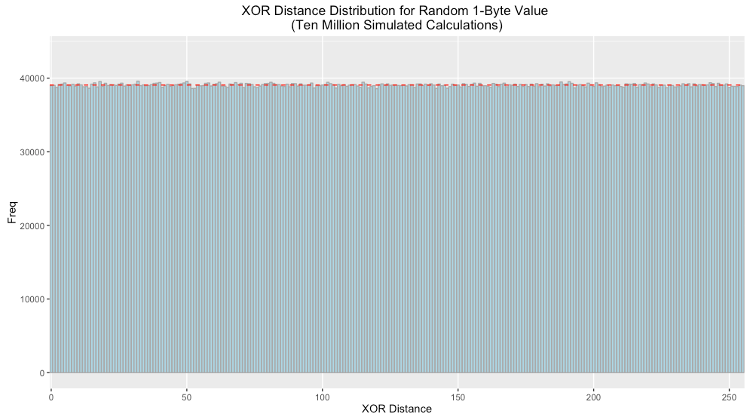
\includegraphics[width=\linewidth]{5}
\end{figure}

S-Buckets that have reached $ S $ bytes cannot store more shards. Farmers can determine if bucket $ L_{n} $ is full during contract negotiation by calculating $ n $ using the data-hash field in the contract, and should reject contracts that would cause them to overfill an S-Bucket. When all buckets in a KFS instance are full, a second instance may be made. Given that the 8 TiB upper limit of a farmer’s KFS instance is larger than most available drives, this is unlikely for most hardware.

\subsubsection{Keying By Shard Hash}
As mentioned earlier, LevelDB sorts items lexicographically by key. KFS takes advantage of this to optimize the efficiency of reads and writes. Data is stored in chunks of $ C $ bytes (or less). By default $ C = 128 $ KiB. These chunks are keyed by the full content's hash followed by a space and a numerical index. This ensures that key/value pairs are small, and that reads and writes to and from a S-Bucket are sequential. It also allows for efficient streaming of data both in and out of the S-bucket.

Because of the idiosyncrasies of sorting numerical strings lexicographically, the index substring should be expressed in base 10, and have a constant number of characters. The length $ l $ of the index string should be defined by $ l = \lceil log_{10} \frac{S}{C} \rceil $. For default parameters $ l = 6 $, meaning that the chunk at index 3753 will have have the index number 003753. This ensures that chunks of a shard are stored consecutively.

To preserve order and therefore maximize read/write performance, the keys for the chunks of a specific shard should be strings generated as follows:

\begin{enumerate}
\item Determine the chunk index number, and encode it as a string.
\item Prepend the chunk index string with '0' until it reaches length $ l $.
\item Encode $ H(data) $ as a string of hexadecimal characters.
\item Append a single space to the hash.
\item Append the modfied chunk index to the hash.
\end{enumerate}

\subsubsection{Performance Benefits}
In initial testing KFS outperforms vanilla LevelDB in reads, writes, and unlinks at a variety of file sizes. KFS displays lower means and lower variance across almost all combinations of file size, operation, and storage device type. It particularly excels at unlinks and writes of large files, reducing variance by several orders of magnitude. The full methodology of these tests, and their results, can be found elsewhere \cite{13}.

%insert Figure 6
\begin{figure}[hbt]
\centering
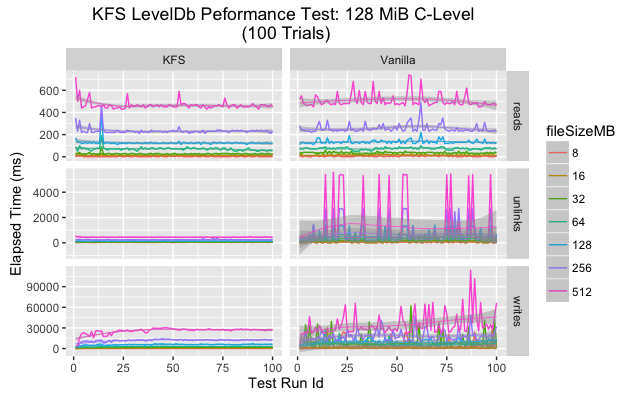
\includegraphics[width=\linewidth]{6}
\end{figure}

\subsection{NAT Traversal and Reverse HTTP Tunneling}
Due to the presence of NATs and other adverse network conditions, not all devices are publicly accessible. To enable non-public nodes to participate in the network, Storj implements a reverse tunnel system.

To facilitate this system, Storj extends Kademlia with three additional message types: PROBE, FIND\_TUNNEL, and OPEN\_TUNNEL The tunneling system also makes use of the publish/subscribe system detailed in section 2.6.

PROBE messages allow a node to determine whether it is publically addressable. The message is sent to a publicly addressable node, typically a known network seed. The receiving node issues a separate PING message. The receiving node then responds to the PROBE message with the result of the PING. Nodes joining the network should immediately send a PROBE to any known node.

Nodes that receive a negative response to their initial PROBE should issue a FIND\_TUNNEL request to any known node. That node must respond with three contacts that have previously published a tunnel announcement via the publish/subscribe system. Tunnel providers must be publicly addressable.

Once the non-public node has received a list of tunnel providers, it issues OPEN\_TUNNEL requests to the tunnel providers. The providers must provide a tunnel for that node if they are capable. To open a connection, the provider sends back an affirmative response with tunnel information. The tunneled node then opens a long-lived connection to the provider, and updates its own contact information to reflect the tunnel address.

Tunnels are operated over TCP sockets by a custom reverse-tunneling library, Diglet \cite{14}. Diglet provides a simple and flexible interface for general-purpose reverse tunneling. It is accessible both by command-line and programmatically.

\subsection{Data Transfer}
Data is transferred via HTTP \cite{15}. Farmers expose endpoints where client applications may upload or download shards. Clients requests are authenticated via tokens provide by previous CONSIGN and RETRIEVE messages. This transfer mechanism is not essential to the protocol, and many alternatives may be implemented in the future.


\section{Network Access}
As should be apparent, the data owner has to shoulder significant burdens to maintain availability and integrity of data on the Storj network. Because nodes cannot be trusted, and hidden information like challenge sets cannot be safely outsourced to an untrusted peer, data owners are responsible for negotiating contracts, pre-processing shards, issuing and verifying audits, providing payments, managing file state via the collection of shards, managing file encryption keys, etc. Many of these functions require high uptime and significant infrastructure, especially for an active set of files. User run applications, like a file syncing application, cannot be expected to efficiently manage files on the network.

To enable simple access to the network from the widest possible array of client applications, Storj implements a thin-client model that delegates trust to a dedicated server that manages data ownership. This is similar to the SPV wallet concept found in Bitcoin and other cryptocurrency ecosystems. The burdens of the data owner can be split across the client and the server in a variety of ways. By varying the amount of trust delegated, the server could also provide a wide variety of other valuable services. This sort of dedicated server, called Bridge, has been developed and released as Free Software. Any individual or organization can run their own Bridge server to facilitate network access.

\subsection{Bridge}
Our reference implementation of this model consists of a Bridge server, and a client library. Bridge provides an object store, which is to say, the primary function of Bridge is to expose an API to application developers. Developers should be able to use the Bridge via a simple client without requiring knowledge of the network, audit procedures, or cryptocurrencies. The Bridge API is an abstraction layer that streamlines the development process. This enables developers to create many applications that use the Storj network, allowing the network to reach many users.

In the current implementation, Bridge assumes responsibility for contract negotiation, audit issuance and verification, payments, and file state, while the client is responsible for encryption, pre-processing, and file key management. The Bridge exposes access to these services through a RESTful API. In this way, the client can be completely naive of the Storj protocol and network while still taking advantage of the network. In addition, because the dedicated server can be relied on to have high uptime, the client can be integrated into unreliable user-space applications.

Bridge is designed to store only metadata, and to never transit or store shards. Bridge cannot cache encrypted shards, and does not hold keys to them. The client maintains complete control over access to the data, regardless of any action Bridge takes. Bridge can expose only metadata like access patterns to third parties.

It is possible to envision Bridge upgrades that allow for different levels of delegated trust. A Bridge client may want to retain control over issuing and validating audits, or managing pointers to shards. Or a client may choose to authorize two or more unrelated Bridges to manage its audits in order to minimize the trust it places in either Bridge server. In the long run, any function of the data owner can be split across two or more parties by delegating trust.

\subsection{Bridge API and Client}
Full documentation of the Bridge API is outside the scope of this whitepaper, but is available elsewhere \cite{16}. The first complete client implementation is in JavaScript. Implementations are in progress in C, Python, and Java.

Because files cannot simply be POSTed to API endpoints, the structures of the Bridge API and client are different from existing object stores. Clients, as much as possible, to hide this from users and application developers by exposing simple, familiar interfaces. Complex network operations should be distilled to individual function calls.

A brief summary of the upload process follows:

\begin{enumerate}
\item The client gathers and pre-processes data.
\item The client notifies Bridge of data awaiting upload.
\item Bridge negotiates contracts with network nodes.
\item Bridge returns the IP addresses of contracted nodes, and authorization tokens to the client.
\item The client uses the IP addresses and tokens to contact the farming nodes and upload the data.
\item The client transfers the audit information to the Bridge, thus delegating trust.
\item Bridge assumes responsibility for issuing audits, paying farmers, and managing file state.
\item Bridge exposes file metadata to the client via the API.
\end{enumerate}

The download process is similar.

\begin{enumerate}
\item The client requests a file by an identifier.
\item Bridge validates the request and provides a list of farmer IP addresses and tokens.
\item The client uses the addresses and tokens to retrieve the file
\item The file is reassembled and decrypted client-side.
\end{enumerate}

The JavaScript library accepts file, handles pre-processing, and manages connections as directed by Bridge. It also makes decrypted downloads available to applications as files, or as streams. A sample CLI using the library is available as Free Software at https://github.com/storj/core-cli. It has been tested with a wide variety of file sizes, and is capable of reliably streaming 1080p video from the Storj network.

\subsubsection{Application Development Tools}
The primary function of Bridge and the Bridge API is to serve applications. To this end clients and tools in a wide variety of languages are under development.

Storj.js seeks to provide a standard in-browser interface for downloading files from Storj. Though in early stages, it can already communicate with Bridge, retrieve file pointers and tokens, retrieve shards from farmers, reassemble shards, and append the completed file to the DOM. This allows web developers to easily reference Storj objects from within a page, and rely on them being delivered properly to the end user. This could be used to provide any service from in-browser document editing to photo storage.

Key and file management tools for web backends are in early planning stages, including Storj plugins for standard backend tools like content management systems. These tools should help content-driven application developers work with files on the Storj network. Standardizing these tools around permissioning files by user could help create data portability between services as discussed in section 4.2.

Bridges to other protocols and workflows are also planned. The Storj CLI lends itself to shell scripting automation. Similar tools for FTP, FUSE, and common tools for interacting with files will be developed in the future.

\subsection{Bridge as an Authorization Mechanism}
Bridge can be used to manage authorization for private files stored on the network. Because Bridge manages the state of each contract under its care, it is a logical provider of these services. It can manage a variety of authorization-related services to enable sharing and collaboration.

\subsubsection{Identity and Permissioning}
The Bridge API uses public-key cryptography to verify clients. Rather than the Bridge server issuing an API key to each user, users register public keys with the Bridge. API requests are signed, and the Bridge verifies that the signature matches a registered public key. Bridge organizes file metadata into buckets to facilitate management. Buckets can be permissioned individually by registering a set of public keys to the Bucket.

Application developers can use this to easily delegate permissions to applications, servers, or  other developers. For instance, the developer of a file syncing service could create a keypair for each user of that service, and divide each user into a separate Bucket accessible only by that user’s keypair. Usage of each Bucket is tracked separately, so users who have exceeded their allotment could have write permissions revoked programmatically. This provides a logical separation of user permissions, as well as a variety of organizational tools.

\subsubsection{Key Migration}
Because shard encryption keys are stored on the device that generated them, data portability is an issue. The reference implementation of Bridge and the client facilitate the transfer of file encryption keys between clients in a safe way. Clients generate a cryptographically strong passphrase, like a twelve word seed. To encrypt a given file the client generates a deterministic key based on the seed, Bucket ID and File ID. The user can then transmit the seed phrase between devices, and rely on Bridge to provide the Bucket ID and File ID.

\subsubsection{Public Files}
Bridge, like other object stores, allows developers to create and disseminate public files via public Buckets. The Bridge server allows the developer to upload the encryption key, and then allows anonymous users to retrieve the file key and the set of file pointers. Public Buckets are useful for content delivery to webpages, or to public-facing applications.

\subsubsection{File Sharing}
In the future, the Bridge could enable sharing of specific files between applications or users. Because all files co-exist on a shared network, this is a problem of standardization and identity management.

Standardization of file and metadata formats could create file portability between applications. Intelligent use of Bridge’s permissioning systems could allow end users to migrate data between many interoperable applications while preserving privacy and data security. A photo stored via a phone syncing service could also be available in a browser-based photo editor offered by an unrelated developer.

Bridge could also use a third-party source of identity, like a PGP keyserver or Keybase, to enable secure person-to-person file sharing. A tiered keying strategy (like Lastpass uses) could also allow for the sharing of individual files. Other cryptographic schemes like proxy re-encryption seem promising. For a simplified example: if file keys are strongly encrypted and escrowed with a Bridge, files could be shared to any social media handle that could be authenticated via Keybase. Bridge could send the corresponding client a single encrypted file key along with a transposition key, thus enabling access to a file without exposing the file to Bridge, or modifying the file in any way.

A thorough description of these key management schemes is outside the scope of this paper. It is enough to note that they exist, that many useful strategies can be implemented in parallel, and that a dedicated Bridge can facilitate them in many useful ways.

\subsection{Bridge as a Network Information Repository}
As noted earlier, data owners are responsible for negotiating contracts and managing file state. With enough information about peers on the network, contract selection becomes a powerful tool for maintaining file state. A Bridge will have many active contracts with many farmers, and will therefore have access to information about those farmers. A Bridge could use this information to intelligently distribute shards across a set of farmers in order to achieve specific performance goals.

For instance, via the execution of a contract, a Bridge node gathers data about the farmer’s communication latency, audit success rate, audit response latency, and availability. With minimal additional effort, the Bridge could also gather information about the node’s available bandwidth. By gathering a large pool of reliable data about farmers, a Bridge node can intelligently select a set of farmers that collectively provides a probabilistic guarantee of a certain quality of service.

In other words, the Bridge can leverage its knowledge about peers on the network to tailor the service to the client’s requirements. Rather than a limited set of service tiers, a Bridge could assemble a package of contracts on the fly to meet any service requirement. This allows the client to determine the optimal latency, bandwidth, or location of a file, and have confidence that its goals will be met. For instance, a streaming video application may specify a need for high bandwidth, while archival storage needs only high availability. In a sufficiently large network, any need could be met.

This function is nearly impossible to distribute, as the retrieval and processing overhead of a distributed network are unsuitable to the high-performance demands of most storage applications. This also cannot be easily replicated by a data-center based object store. In a distributed network, knowledge about the network is incredibly valuable.

\subsection{Bridge as a Service}
In cases where the cost of delegating trust is not excessively high, clients may use third-party Bridges. Because Bridges do not store or transit data and have no access to keys, this is still a large improvement on the traditional data-center model. Many of the features Bridge servers provide, like permissioning and intelligent contracting, leverage considerable network effects. Larger data sets create far better performance for clients.

Applications using object stores delegate significant amounts of trust to the storage providers. Providers may choose to operate public Bridges as a service. Application developers then delegate trust to the Bridge, exactly as they would to a traditional object store. This shifts significant operational burdens from the application developer to the service-provider with minimal trust delegation. This would also allow developers to pay for storage with standard payment mechanisms, like credit cards, rather than managing a cryptocurrency wallet. Storj Labs Inc. currently provides this service.


\section{Future Areas of Research}
Storj is a work in progress, and many features are planned for future versions. There are relatively few examples of functional distributed systems at scale, and many areas of research are still open.

\subsection{Federated Bridges}
Bridge nodes could cooperate to share data about the network in a mutually beneficial federation. This would allow each Bridge to improve the quality of service that it provides by improving the quality of information available.

Bridges could also, with the consent of users, cooperate to share file metadata and pointers among themselves. This would allow a user to access their file from any Bridge, rather than being dependent on a single Bridge. A tiered set of fallback Bridges storing the same access information is a desirable feature, as it hedges against downtime from a solo Bridge. Some solvable permissioning issues may exist, but there is no reason to believe a standard format and algorithm for syncing state across Bridges may not be developed.

\subsection{Data Portability}
By encouraging use of data format and access standards, Storj aims to allow portability of data between applications. Unlike a traditional model, where control of data is tied to the service used to access the data, data access may be tied to individual users because Storj forms a common underlying layer. User data can be tied to persistent cryptographic identities, and authenticated without exposing data to third parties. Siloing data in applications is a harmful relic of traditional models. Building cross-compatibility into the future of data storage greatly improves user privacy and user experience.

Applications implementing these standards would be broadly compatible. When access is tied to users rather than services, privacy and control are preserved. A user may grant access to a service that backs up their hard drive, which places those files in Storj. The user could separately grant access to a photo-sharing service, which could then access any photos in the backup. The user gains seamless portability of data across many applications, and application developers gain access to a large pool of existing users.

Permissioning in this system may be managed by a service like a Bridge, tied to a web of trust identity via services like Keybase, or handled by a distributed self-sovereign identity system. Smart contract systems, e.g. Ethereum \cite{17} contracts, seem like a sensible long-term choice, as they can provide file permissions based on arbitrary code execution. Some problems may exist with respect to management of the private information required for identity and permissioning systems, but sufficient solutions likely exist.

While this system represents a significant step up in both usability and value, there are unmitigable security issues. Unfortunately, as in any cryptographic system, it is impossible to revoke access to data. Applications may cache data or forward it to third parties. Users, by definition, trust application developers to handle their data responsibly. To mitigate these risks, Storj Labs intends to provide incentives to developers to build free and open-source software. No application can be completely secure, but auditable code is the best defense of user’s privacy and security.

The potential advantages in terms of user experience and privacy are great, but more research is needed. Many open questions exist with respect to permissioning mechanisms,  At worst a unified backend powering interoperable applications provides equivalent security to current data-center based models. Storj hopes to collaborate with other forward-thinking data-driven projects to create and advocate for these open standards.

\subsection{Reputation Systems}
Storj, like many distributed networks, would profit immensely from a distributed reputation system. A reliable means of determining reputation on a distributed system is an unsolved problem. Several approaches have been detailed, and some implemented in practice, but none have achieved consensus among researchers or engineers. A brief review of several of these approaches follows.

One inherent downside of distributing information across a network is the additional latency required for decisionmaking. It is difficult to say whether any distributed reputation system can accurately assess the bandwidth, latency, or availability of peers on a distributed network in a manner suitable to object storage, especially as market demand for these shifts over time. Nevertheless, a reliable distributed reputation would be an extremely useful tool for interacting with and understanding the network.

\subsubsection{IPFS Bitswap}
IPFS presents the concept of BitSwap ledgers \cite{18}. BitSwap ledgers are simple local accounting of past interactions with other nodes. As IPFS and the BitSwap protocols are primarily concerned with distribution of objects in a Kademlia-style DHT, BitSwap ledgers counts bytes sent and bytes received. Rather than attempt to reach global consensus about the reputation state of the system, these ledgers deal only with one-to-one relationships, and do not account for latency, bandwidth, availability, or other quality of service factors. Most of the behavior of nodes is left to the implementer, with some discussion given to potential exchange strategies. This implies that BitSwap ledgers scale well and are extremely versatile.

\subsubsection{Eigentrust and Eigentrust++}
Eigentrust \cite{19} attempts to generalize the ledger approach to generate global trust values in a distributed system using a transitive-trust model. Nodes keep and exchange trust vectors. For networks with a large majority of trustworthy peers, the value of each local trust vector converges to a shared global trust vector as nodes learn more about the network via information exchange.

Eigentrust++ \cite{20} identifies several attack vectors and modifies Eigentrust to improve performance and reliability in the presence of malicious nodes. Eigentrust++ is currently implemented in NEM \cite{21}.  Secure global convergence to a shared trust value for each node is a key feature for any distributed reputation system.

\subsubsection{TrustDavis}
TrustDavis \cite{22} implements reputation as insurance. Nodes provide references for other nodes in the form of insurance contracts. Nodes seeking a prospective partner for an economic transaction also seek insurance contracts protecting them from the actions of that partner. Reputation in this system may be thought of as a graph, with vertices representing nodes, and directed edges representing the monetary value that a node is willing to stake on behalf of another. Nodes that are distant in this graph may still transact by purchasing a set of insurance contracts that traverses these edges. TrustDavis in practice thus encounters the same routing problem found on other distributed systems like the Lightning Network.

Denominating trust in terms of monetary value is attractive for an economic network like Storj, but the mechanics of insurance contracts in a system like this represent an extremely difficult problem.  Notably, because failures to deliver payment propagate backwards through the insurance route, the financial burden always falls on the node that trusted an untrustworthy node, rather than the untrustworthy nodes.

\subsubsection{Identity Maintenance Costs}
Storj is exploring a reputation system that leverages public Blockchains to solve a narrow set of identity problems \cite{23}. This system relies on miners’ fees as a substitute for proof-of-burn. Nodes invest in their identity over time by making small standardized payments to their own Storj network node ID. Because the ID is a Bitcoin address to which the node holds the private key, these funds are fully recoupable, except for the miners’ fee. In this system, nodes prefer to interact with nodes that have a long history of regular transactions. Regular transactions over time indicate monetary investment in an identity equal to the sum of the miners’ fees paid.

The payment required to participate in this system should be significantly less than the expected return of operating a network node. If set correctly, this recurring monetary payment for an identity bounds the size and duration of Sybil attacks without affecting cooperative nodes. Legitimate nodes would easily recoup their identity expense, while Sybil operators would find their expenses outstripping their returns. This approach solves a relatively small subset of identity issues on the network, and it is difficult to see how it could be extended to other problem sets.

\subsection{OFFER Loop Strategies}
Many negotiation strategies can exist and interact via the OFFER loop. Full exploration of negotiation strategies is beyond the scope of this paper, but a few interesting areas are immediately apparent. Simple examples include price floors and ceilings, but complex models could be built to base strategies on market trends and the subjective value of a shard. Negotiation strategies executed by autonomous agents are an area of (fascinating) ongoing research. Storj will be one of the first large-scale machine-driven marketplaces. As such, improving negotiation efficiency is critical to the long-term efficiency of the market.

\section{Attacks}
As with any distributed system, a variety of attack vectors exist. Many of these are common to all distributed systems. Some are storage-specific, and will apply to any distributed storage system.

\subsection{Spartacus}
Spartacus attacks, or identity hijacking, are possible on Kademlia. Any node may assume the identity of another node and receive some fraction of messages intended for that node by simply copying its Node ID. This allows for targeted attacks against specific nodes and data. This is addressed by implementing Node IDs as ECDSA public key hashes and requiring messages be signed. A Spartacus attacker in this system would be unable to generate the corresponding private key, and thus unable to sign messages and participate in the network.

\subsection{Sybil}

Sybil attacks involve the creation of large amounts of nodes in an attempt to disrupt network operation by hijacking or dropping messages. Kademlia, because it relies on message redundancy and a concrete distance metric, is reasonably resistant to Sybil attacks. A Node’s neighbors in the network are randomly selected by Node ID, and most messages are sent to at least three neighbors. If a Sybil attacker controls 50\% of the network, it successfully isolates only 12.5\% of honest nodes. While reliability and performance will degrade, the network will still be functional until a large portion of the network consists of colluding Sybil nodes.

\subsubsection{Google}
The Google attack, or nation-state attack, is a hypothetical variant of the Sybil attack carried out by an entity with extreme resources. Google attacks are hard to address, as it is difficult to predict the actions of an organization with orders of magnitude more resources than the sum of the resources of network participants. The only reliable defence against a Google attack is to create a network whose resources are on the same order of magnitude as the attacker’s. At that scale, any attack against the network would represent an unsustainable commitment of resources for such an organization.

\subsubsection{Honest Geppetto}
The Honest Geppetto attack is a storage-specific variant of the Google attack. The attacker operates a large number of ‘puppet’ nodes on the network, accumulating trust and contracts over time. Once he reaches a certain threshold he pulls the strings on each puppet to execute a hostage attack with the data involved, or simply drops each node from the network. Again, the best defence against this attack is to create a network of sufficient scale that this attack is ineffective. In the meantime, this can be partially addressed by relatedness analysis of nodes. Bayesian inference across downtime, latency and other attributes can be used to assess the likelihood that two nodes are operated by the same organization, and data owners can and should attempt to distribute shards across as many unrelated nodes as possible.

\subsection{Eclipse}
An eclipse attack attempts to isolate a node or set of node in the network graph, by ensuring that all outbound connections reach malicious nodes. Eclipse attacks can be hard to identify, as malicious nodes can be made to function normally in most cases, only eclipsing certain important messages or information. Storj addresses eclipse attacks by using public key hashes as Node IDs. In order to eclipse any node in the network, the attacker must repeatedly generate key pairs until it finds three keys whose hashes are closer to the targeted node than its nearest non-malicious neighbor, and must defend that position against any new nodes with closer IDs. This is, in essence, a proof-of-work problem whose difficulty is proportional to the number of nodes in the network. For large networks it becomes prohibitively expensive to perform an eclipse attack (see Section 6.2). Furthermore, any node that suspects it has been eclipsed may trivially generate a new keypair and node ID, thus restarting the proof-of-work challenge.

\subsubsection{Tunnel Eclipse}
Because tunneled connections rely on the tunnel provider, it is trivial for a tunnel provider to eclipse nodes for which it provides tunneled connections. This attack cannot affect publicly addressable nodes, so it can be trivially defeated with proper configuration. This attack can be mitigated by encrypting messages intended for tunneled nodes, thus removing the malicious tunnel provider's ability to inspect and censor incoming messages. Like a typical eclipse attack, any node that suspects it is the victim of a tunnel eclipse can easily generate a new Node ID, and find a new tunnel.

\subsection{Hostage Bytes}
The hostage byte attack is a storage-specific attack where malicious farmers refuse to transfer shards, or portions of shards, in order to extort additional payments from data owners. Data owners should protect themselves against hostage byte attacks by storing shards redundantly across several nodes (see Section 2.7). As long as the client keeps the bounds of its erasure encoding a secret, the malicious farmer cannot know what the last byte is. Redundant storage is not a complete solution for this attack, but addresses the vast majority of practical applications of this attack. Defeating redundancy requires collusion across multiple malicious nodes, which is difficult to execute in practice.

\subsection{Cheating Owner}
A data owner may attempt to avoid paying a farmer for data storage by refusing to verify a correct audit. In response the farmer may drop the data-owner’s shard. This attack primarily poses a problem for any future distributed reputation system, as it is difficult for outside observers to verify the claims of either party. There is no known practical publicly verifiable proof of storage, and no known scheme for independently verifying that a privately verifiable audit was issued or answered as claimed. This indicates that a cheating client attack is a large unsolved problem for any reputation system.

\subsection{Faithless Farmer}
While the farming software is built to require authentication via signature and token before serving download requests, it is reasonable to imagine a modification of the farming software that will provide shards to any paying requestor. In a network dominated by faithless farmers, any third-party can aggregate and inspect arbitrary shards present on the network.

However, even should faithless farmers dominate the network, data privacy is not significantly compromised. Because the location of the shards that comprise a given file is held solely by the data owner, it is prohibitively difficult to locate a target file without compromising the owner (see Section 6.3). Storj is not designed to protect against compromised data owners. In addition, should a third-party gather all shards, strong client-side encryption protects the contents of the file from inspection. The pointers and the encryption key may be secured separately. In the current implementation of Bridge, the pointers and the keys are held by the Bridge and the client, respectively.

\subsection{Defeated Audit Attacks}
A typical Merkle proof verification does not require the verifier to know the depth of the tree. Instead the verifier is expected to have the data being validated. In the Storj audit tree, if the depth is unknown to the verifier the farmer may attack the verification process by sending a Merkle proof for any hash in the tree. This proof still generates the Merkle root, and is thus a valid proof of some node. But, because the verifier does not hold the data used to generate the tree, it has no way to verify that the proof is for the specific leaf that corresponds to the challenge. The verifier must store some information about the bottom of the tree, such as the depth of the tree, the set of leaves nodes, or the set of pre-leaves. Of these, the depth is most compact, and thus preferable.

Using the pre-leaf as an intermediary defeats another attack, where the farmer simply guesses which leaf corresponds to the current challenge. While this attack is unlikely to succeed, it’s trivially defeated by forcing the farmer to provide the pre-leaf. The farmer cannot know the pre-leaf before the challenge is issued. Requiring transmission of the pre-leaf also allows the data owner to proceed through the challenge set linearly instead of being forced to select randomly. This is desireable because it allows the data owner to maintain less state information per tree.

\section{Selected Calculations}
The following are several interesting calculations related to the operation of the network.

\subsection{Failure of k-of-n Erasure Coding}
The chance of failure of k-of-n erasure coding failing assuming probability $ p $ every shard stays online, is calculated as a binomial distribution:

{\centering
$\Pr_{failure}(n; k,p) = \displaystyle \sum_{i=0}^{k-1} p^{k}(1-p)^{n-k }{n \choose k}$
\\}

%code formatting
\begin{table}[hbt!]
\begin{center}
\begin{tabular}{r r l r}
n & k & p & $\Pr_{failure}{n,k,p}$\\
\hline  18& 6&   0.5  & 4.812e-02\\
\hline  18& 6&   0.75&3.424e-05\\
\hline  18& 6&   0.9  & 5.266e-10\\
\hline  18& 6&   0.98&6.391e-19\\
\hline  36& 12& 0.5  &1.440e-02\\
\hline  36& 12&  0.75&2.615e-08\\
\hline  36& 12&  0.9  &1.977e-17\\
\hline  36& 12&  0.98&1.628e-34\\
\end{tabular}
\end{center}
\end{table}

Code:
\begin{lstlisting}
def fac(n): return 1 if n==0 else n * fac(n-1)
def choose(n,k): return fac(n) / fac(k) / fac(n-k)
def prob(n,k,p): return choose(n,k) * p ** k * (1-p) ** (n-k)
def prob_fail(n,k,p): return sum([prob(n,i,p) for i in range(0,k)])
\end{lstlisting}

Therefore, with well-chosen $ k $ and $ n $, in addition to recovery methods described above, the statistical chance of shard or file loss is quite small.

\subsection{Difficulty of Eclipsing a Target Node}
The probability of eclipsing a targeted node in the a network with $ i $ nodes in $ h $ hashes is modeled by a similar binomial distribution:

{\centering
$\Pr_{success}(h, i) = \displaystyle \sum_{k=3}^{h-1} (i)^{-k}(1-\frac{1}{i})^{h-k}{k \choose h}$
\\}

%TODO table

Code:
\begin{lstlisting}
def fac(k): return 1 if k==0 else k * fac(k-1)
def choose(h,k): return fac(h) / fac(k) / fac(h-k)
def prob(k,h,i): return choose(h,k) * i ** -k * (1-(1.0/i)) ** (h-k)
def prob_succ(h,i): return sum([prob(k,h,i) for k in range(3,h)])
\end{lstlisting}



\subsection{Beach Size}
As the number of shards on the network grows, it becomes progressively more difficult to locate a given file without prior knowledge of the locations of its shards. This implies that even should all farmers become faithless, file privacy is largely preserved.

The probability of locating a targeted file consisting of $ k $ shards by $ n $ random draws from a network containing $ N $ shards is modeled as a hypergeometric distribution with $ K = k $:

{\centering
$Pr_{Success}(N,k,n) = \displaystyle \frac{{N-k \choose n-k}}{{N \choose n}}$
\\}

%TODO: table

Code:
\begin{lstlisting}
def fac(k): return 1 if k==0 else k * fac(k-1)
def choose(k,h): return fac(k) / fac(h) / fac(k-h)
def prob(N,K,n,k): return choose(N-K, n-k) / choose(N,n)
def prob_success(N,k,n): return prob(N,k,n,k)
\end{lstlisting}

\subsection{Partial Audit Confidence Levels}
Farmers attempting to game the system may rely on data owners to issue partial audits. Partial audits allow false positives, where the data appears intact, but in fact has been modified. Data owners may account for this by ascribing confidence values to each partial audit, based on the likelihood of a false positive. Partial audit results then update prior confidence of availability. Data owners may adjust audit parameters to provide desired confidence levels.

The probability of a false positive on a parital audit of $ n $ bytes of an $ N $ byte shard, with $ K $ bytes modified adversarially by the farmer is a hypergeometric distribution with $ k = 0 $:

{\centering
$Pr_{false positive}(N,K,n) = \displaystyle \frac{{N-K \choose n}} {{N \choose n}}$
\\}

%TODO: table

Code:
\begin{lstlisting}
def fac(k): return 1 if k==0 else k * fac(k-1)
def choose(k,h): return fac(k) / fac(h) / fac(k-h)
def prob(N,K,n,k): choose(N-K, n-k) / choose(N,n)
def prob_false_pos(N,K,n): return prob(N,K,n,0)
\end{lstlisting}

\newpage
\appendix
\section{List of Storj Message Types}
\subsection{Kademlia}
\begin{enumerate}
\item PING - Determine whether a node is online.
\item STORE - Store a value in the DHT.
\item FIND\_NODE - Find a node in the DHT.
\item FIND\_VALUE - Find a value in the DHT.
\newcounter{enumTemp}
\setcounter{enumTemp}{\theenumi}
\end{enumerate}
\subsection{Tunneling}
\begin{enumerate}
\setcounter{enumi}{\theenumTemp}
\item PROBE - Determine whether the sender is publicly addressable.
\item FIND\_TUNNEL - Find a publicly addressable node offering tunnels.
\item OPEN\_TUNNEL - Open a tunnel with a node offering tunnels.
\setcounter{enumTemp}{\theenumi}
\end{enumerate}
\subsection{Quasar}
\begin{enumerate}
\setcounter{enumi}{\theenumTemp}
\item SUBSCRIBE - Request filter lists from neighbors.
\item UPDATE - Notify neighbors of updated filters.
\item PUBLISH - Broadcast a message to interested nodes.
\setcounter{enumTemp}{\theenumi}
\end{enumerate}
\subsection{Contracting}
\begin{enumerate}
\setcounter{enumi}{\theenumTemp}
\item OFFER - Propose or finalize a contract.
\item CONSIGN - Request a PUSH token from a farmer.
\item MIRROR - Instruct a farmer to retrieve and mirror data from another farmer.
\item AUDIT - Issue an audit challenge to a farmer.
\item RETRIEVE - Request a PULL token from a farmer.
\end{enumerate}


\newpage
\bibliographystyle{unsrt}
\begingroup
  \raggedright
  \bibliography{Storj2}
\endgroup


\end{document}
